\documentclass{article}

\usepackage{floatrow}
\usepackage{graphicx} % Required for inserting images
\usepackage[a4paper, total={6in, 8in}]{geometry}
\usepackage{parskip} % Required to stop indenting new paragraphs
\usepackage{amssymb}
\usepackage{amsmath}
\usepackage{algpseudocode}
\usepackage{algorithm}
\usepackage{pgfplotstable}
\usepackage{arydshln} % dashed lines in tables
\usepackage[numbers]{natbib} % number references and natbib for more styles
\bibliographystyle{unsrtnat} % sets bibliography to vancouver style

\title{Reverse Mode Algorithmic Differentiation}
\author{Callum Firth, Maximilian Fricker, Alexander Le Marchant, Samuel Murdoch} % alphabetical
\date{}

\begin{document}

\maketitle

\tableofcontents
\newpage

\section{Introduction}

Complex computer simulations and models underpin our modern society - being at the heart of a vast number of endeavours such as weather forecasting, modelling of the spread of disease and machine learning. These models often rely on the computation of a large number of derivatives in order to assess how changing certain parameters affects the outputs in order to optimise the system. This means that being able to differentiate these programs with a method that is both fast and efficient is very important. The technique we explore in this report to do this is algorithmic differentiation.

Algorithmic differentiation is essential to the training of neural networks. Neural networks consist of many nodes connected by a series of weights that can be adjusted in order to change the output of the model. The algorithm that is most commonly used to do this is gradient descent. The goal of gradient descent is to find a local minimum of a cost function that measures the distance between the data predicted by the model and the observed results. It does this by computing the derivative of the cost function with respect to model parameters and then adjusting those parameters such that the derivative reduces in magnitude to get closer to the optimal model. As neural networks are often controlled by thousands or millions of parameters, it is imperative that a fast method of differentiation is used.

During the computation of computer models and simulations, it is often necessary to solve non-linear systems of equations as the vast majority of real-world systems are not linear. However, in general, it is very difficult to directly solve these systems and so they have to be solved numerically. One such method is Newton's method which relies on calculating derivatives. Say the system is defined by
\begin{equation} \label{Fxy}
        F: \mathbb{R}^n \rightarrow \mathbb{R}^m \quad F(x_1, \cdots, x_n) = (y_1, \cdots, y_m)
\end{equation}
then given $x_0 \in \mathbb{R}^n$ the iterates are calculated by
\begin{equation}
x_{n+1} = x_n - (F'(x_n))^{-1}F(x_n) \quad n \in \mathbb{N}
\end{equation}
where $F'(x_n)$ is the Jacobian of $F$ at $x_n$ defined by
\begin{equation} \label{jacobian}
    F'(x) = \begin{bmatrix}
        \frac{\partial y_1}{\partial x_1} & \cdots & \frac{\partial y_1}{\partial x_n} \\
        \vdots & \ddots & \vdots \\
        \frac{\partial y_m}{\partial x_1} & \cdots & \frac{\partial y_m}{\partial x_n}
    \end{bmatrix} \in \mathbb{R}^{m \times n}
\end{equation}

Hence finding the derivative of a function is essential for us to be able to solve our system. So we need to find a way of computing the derivative of a function at low cost due to the fact that a high number of iterates will need to be calculated.

From these examples and those stated in \cite{appad} we see the importance of the implementation of quick derivative computation on computers.

\section{Basics of Computing Derivatives}

There are three common ways to differentiate a function on a computer: numerically, symbolically, and algorithmically. The latter which we will be discussing in depth in this paper. Notably focusing on reverse mode algorithmic differentiation (AD). In contrast to symbolic and algorithmic differentiation, numerical differentiation results in an approximation for the derivative.

The most common example of numerical differentiation is the finite differences method. For \\ $F: \mathbb{R}^n \longrightarrow \mathbb{R}^m$ in \eqref{Fxy}, a partial derivative can be approximated using a truncated Taylor series around $p \in \mathbb{R}^n$. 
\begin{equation}
    \frac{\partial F_i (p)}{\partial x_j} \approx \frac{F_i(p+he_j) - F_i(p)}{h}
\end{equation}
This calculation for the derivative is approximate due to the error in the truncated Taylor series. The computational cost of calculating the Jacobian of $F$ in \eqref{jacobian} is $n + 1$ times the cost of evaluating $F$ \cite{chem}. Thus, finite differences is unsuited for systems with a large number of unknowns.

Symbolic differentiation involves taking an algebraic expression and computing its derivative with respect to a specified variable through repeated application of basic rules of calculus using computer algebra tools. It can be useful as, once the formula for the derivative is computed, finding the value of the derivative at a point is as simple as substituting it into the formula for the derivative.  Furthermore, symbolic differentiation provides an explicit formula for the derivative which is beneficial from a mathematical point of view. However, it has the drawback that it can only be applied when the function to be differentiated exists in a closed form. For calculating the gradient of $F_i$ in \eqref{Fxy}, symbolic differentiation has a computational cost of $n$ times the cost of evaluating $F_i$ \cite{chem}. Hence, the computational cost for calculating the Jacobian of a set of equations, defined by $F$, would be prohibitively expensive at $mn$ times the cost of evaluating $F$.

There are two forms of algorithmic differentiation: forward mode and reverse mode. Fundamental to AD is the application of the chain rule. Both have similar computational costs for the Jacobian but are suited to different types of functions. With forward mode algorithmic differentiation, this has computational cost proportional to $n$ times the cost of evaluating $F$. In contrast, the computational cost of $[F'(x)]^\top$ with reverse mode algorithmic differentiation is proportional to $m$ times the cost of evaluating $F$ \cite{falisse}. Hence, reverse mode is suited for functions $F$ where $n >> m$. We will see below that the reverse mode has an even better complexity error for calculating gradients compared to the alternatives. One drawback of reverse mode algorithmic differentiation over forward-mode is that it requires higher memory usage, due to the necessity to store intermediary values.

\section{Directed Acylic Graphs to Represent Expressions}

For a function $F: \mathbb{R}^3 \rightarrow \mathbb{R}^2$ defined by
\begin{equation} \label{example1}
    F \begin{pmatrix}
        x \\ y \\ z
    \end{pmatrix} = \begin{pmatrix}
        \sin (x^2 y) + e^{x^2} \\ e^{x^2} \log z
    \end{pmatrix}
\end{equation}
its representation as a DAG and an expression tree can be seen in Figure \ref{fig:DAGgraph2}.

\begin{figure}[h]
    \centering
    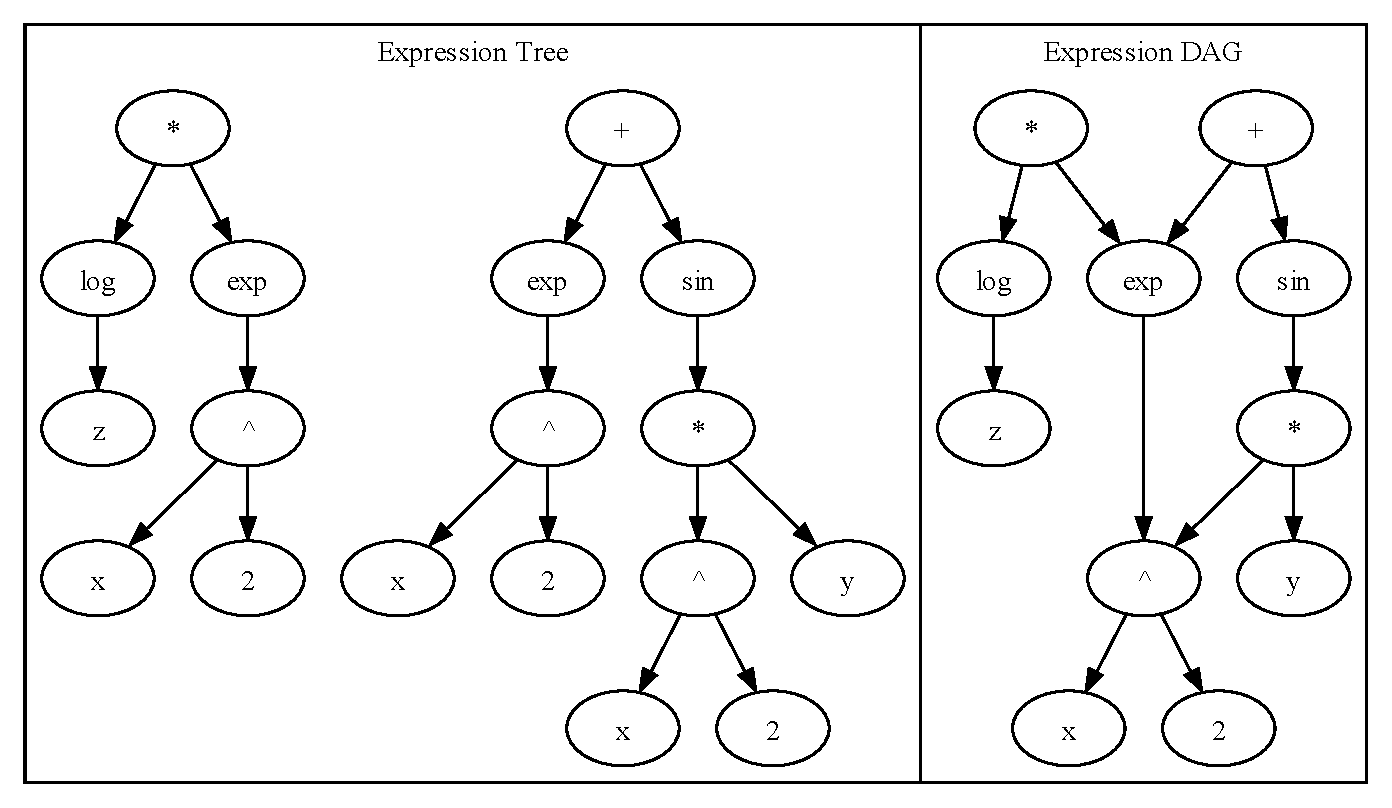
\includegraphics[width=12cm]{images/Graph_Cluster_1.pdf}
    \caption{A DAG and expression tree representation of \eqref{example1}}
    \label{fig:DAGgraph2}
\end{figure}

As in \cite{PoPBook}, we can represent an arithmetic expression as an expression tree. Here we represent each operator, symbol and number in an given expression as nodes in a graph, we denote these as elements. The operands of each element are the children of the node. We will represent links out of a node indicating the children of the node, even though expression wise the children are "inputs" to such parent. We can also write an expression as a directed acylic graph which allows us to represent expressions with more than one operators to avoid recursion. An example of the difference between the two can be see in Figure \ref{fig:DAGgraph2}. We from now on will use DAG's to represent expressions as this is essential in lowering runtime and allowing fast computation of complicated expressions. We will presume that ordering of each child is important.

\section{Fundamentals of Algorithmic Differentiation}

Using notation from \cite{evald}, let $F: \mathbb{R}^n \rightarrow \mathbb{R}^m$ and $F(x) = y$ as in Section 2. Assume $F$ is the composition of a sequence of continuously differentiable elemental functions $(\varphi_i)_{i=1,\ldots, l}$, the derivatives of which can be easily calculated. Hence, $F$ can be represented as a DAG. In our case we will use the elemental functions provided in Table \ref{tab:elemental}.

\begin{table}[h]
    \centering
    \begin{tabular}{|lll|}
        \hline
        Elementary Function $\varphi_i$ & $\partial \varphi_i / \partial {v}_1$ & $\partial \partial \varphi_i / \partial {v}_2$ \\
        \hline
        $v_1+v_2$ & $1$ & $1$ \\
        $v_1-v_2$ & $1$ & $-1$ \\
        $v_1 \times v_2$ & $v_2$ & $v_1$ \\
        $v_1 / v_2$ & $1/v_2$ & $-v_1/v_2^2$ \\
        ${v_1}^{v_2}$ & $v_2{v_1}^{(v_2-1)}$ & ${v_1}^{v_2}\log(v_1)$ \\
        \hdashline
        $\sin(v_1)$ & $\cos(v_1)$ & \\
        $\cos(v_1)$ & $-\sin(v_1)$ & \\
        $\exp(v_1)$ & $\exp(v_1)$ & \\
        $\log(v_1)$ & $1/v_1$ & \\
        \hline
    \end{tabular}
    \caption{Partial Derivatives of Elemental Functions $\varphi$}
    \label{tab:elemental}
\end{table}

The quantities calculated at each node of the graph during the function evaluation are labelled such that
\begin{equation}
    [ \underbrace{v_{1-n}, \ldots, v_0}_{x} , v_1, \ldots, v_{l-m}, \underbrace{v_{l-m+1}, \ldots, v_l}_{y}]
\end{equation}
Using $j \prec i$ to show $v_i$ depends directly on $v_j$ and $j \prec i \Longrightarrow j < i$ then it can be written
\begin{equation}
    v_i = \varphi_i (v_j)_{j \prec i} \text{ for } \varphi_i : \mathbb{R}^{n_i} \longrightarrow \mathbb{R}
\end{equation}

Where we denote $\mathbb{R}^{n_i}$ depends on $\varphi$. Usually here we have that $n=2$ or $n=1$ however later we consider examples where this may not be the case

\subsection{Forward Mode}

We will use the interpretation of forward mode AD given in \cite{dhamarticle}. Assume $x$ is equal to the value a time-dependent $x(t)$ takes at $t=0$. Then define the tangent 
\begin{equation}
    \dot{x} = \frac{\partial x}{\partial t} \Big|_{t=0}
\end{equation}
As $y = F(x)$ we calculate the tangent $\dot{y}$ as
\begin{equation}
    \Dot{y} = \frac{\partial}{\partial t} F(x (t)) \Big|_{t=0} 
    = F'(x (t)) \frac{\partial x}{\partial t} \Big|_{t=0}
    = F'(x) \Dot{x}
    \equiv \Dot{F}(x, \Dot{x})
\end{equation}
Using the additional notation $u_i = (v_j)_{j \prec i}$ and $\Dot{u}_i = (\Dot{v}_j)_{j \prec i}$, the idea can be applied to an elemental function $\varphi_i : \mathbb{R}^{n_i} \longrightarrow \mathbb{R}$, $v_i = \varphi_i (u_i)$ to get the result
\begin{equation} \label{tangentequ}
    \Dot{v_i} = \sum_{j \prec i} \left\{ \Dot{v}_j \cdot \frac{\partial}{\partial v_j} \varphi_i (u_i) \right\} 
    \equiv \Dot{\varphi}_i(u_i, \Dot{u}_i)
\end{equation}

This can be summarised as the general evaluation procedure given in \cite{evald} and given in Table \ref{tab:gep}.
This shows the assignment for all the input, intermediate and output variables

\begin{table}[h]
    \centering
    \begin{tabular}{|lcll|}
        \hline
        $v_{i-n}$ & $\equiv$ & $x_i$ & $i = 1, \ldots, n$ \\
        \hline
        $v_{i}$ & $\equiv$ & $v_i = \varphi_i (u_i)$ & $i = 1, \ldots, l$ \\
        \hline
        $v_{l-m+i}$ & $\equiv$ & $y_i$ & $i = 1, \ldots, m$ \\
        \hline
    \end{tabular}
    \caption{General Evaluation Procedure}
    \label{tab:gep}
\end{table}

Because in forward mode we can calculate both the values and the tangents of our elementary function at the same time we can get a more concise procedure for computing the tangents of our function. This is given in Table \ref{tab:gtp}

\begin{table}[h]
    \centering
    \begin{tabular}{|lcll|}
        \hline
        $[v_{i-n}, \Dot{v}_{i-n}]$ & $=$ & $[x_{i}, \Dot{x}_{i}]$ & $i = 1, \ldots, n$ \\
        \hline
        $[v_{i}, \Dot{v}_{i}]$ & $=$ & $[\varphi_i (u_i), \Dot{\varphi}_i(u_i, \Dot{u}_i)]$ & $i = 1, \ldots, l$ \\
        \hline
        $[v_{l-m+i}, \Dot{v}_{l-m+i}]$ & $=$ & $[y_{i}, \Dot{y}_{i}]$ & $i = 1, \ldots, m$ \\
        \hline
    \end{tabular}
    \caption{General Tangent Procedure}
    \label{tab:gtp}
\end{table}

\subsection{Reverse Mode}

As in \cite{dhamarticle}, consider for the image of $F$ the hyperplane $\{ y \in \mathbb{R}^m | \Bar{y}^\top y = c\}$ for a given vector $\Bar{y} \in \mathbb{R}^m$ and a given value $c \in \mathbb{R}$. The inverse image of this hyperplane is given by the set $\{ x \in \mathbb{R}^n | \Bar{y}^\top F(x) = c\}$. We can apply the implicit function theorem to this set to calculate the normal to this hyperplane at $x$ as
\begin{equation}
    \Bar{x}^\top = \Bar{y}^\top F'(x) \equiv \Bar{F}(x, \Bar{y})
\end{equation}
This calculation is provided $\Bar{x}^\top$ does not vanish.

Using the additional notation $\Bar{u}_i = (\Bar{v}_j)_{j \prec i}$, we calculate the adjoint function for each elemental function $\varphi_i : \mathbb{R}^{n_i} \longrightarrow \mathbb{R}$ as
\begin{equation}
    \Bar{u}_i += \Bar{v}_i \nabla \varphi_i (u_i)
\end{equation}

\begin{equation}
    \Bar{v}_j = \sum_{i \succ j} \left\{ \Bar{v}_i \cdot \frac{\partial}{\partial v_j} \varphi(u_i) \right\}
\end{equation}

In reverse mode, the tree is first traversed beginning at the inputs and finishing at the outputs, storing the value the elemental function takes at each node. Then, the tree is traversed in the other direction storing the value the adjoint function takes at each node. This produces a the adjoint procedure for computing the first derivative from \cite{dhamarticle}, given in Table \ref{tab:ap}.

\begin{table}[h]
    \centering
    \begin{tabular}{|llll|}
        \hline
        $v_{i}$ & $=$ & $0$ & $i = 1, \ldots, l$ \\
        \hline
        $[v_{i-1}, \Bar{v}_{i-1}]$ & $=$ & $[x_{i}, \Bar{x}_{i}]$ & $i = 1, \ldots, n$ \\
        \hline
        push$(v_i)$ & & & \\
        $v_{i}$ & $=$ & $v_i = \varphi_i (u_i)$ & $i = 1, \ldots, l$ \\
        \hline
        $v_{l-i}$ & $=$ & $y_{m-1}$ & $i = 1, \ldots, m-1$ \\
        $\Bar{v}_{l-i}$ & $=$ & $\bar{y}_{m-1}$ & $i = 1, \ldots, m-1$ \\
        \hline
        $v_i \leftarrow$ pop$()$ & & & \\
        $\Bar{u}_i$ & $+=$ & $\Bar{v}_i \nabla \varphi_i (u_i)$ & $i = l, \ldots, 1$ \\
        $v_i$ & $=$ & $0$ & \\
        \hline
        $\Bar{v}_{i-n}$ & $=$ & $\Bar{x}_i$ & $i = 1, \ldots, n$ \\
        \hline
    \end{tabular}
    \caption{General Adjoint Procedure}
    \label{tab:ap}
\end{table}

\section{Complexity Results for Algorithmic Differentiation}

Below we will use notation and results from \cite{dhamarticle} for the number of operations and the memory usage required to compute a function. The number of operations is denoted $\text{OPS}(\cdot)$. The amount of random access memory and the amount of sequentially accessed memory are denoted $\text{RMEM}(\cdot)$ and $\text{SMEM}(\cdot)$ respectively. 

\subsection{Forward Mode}

Given $x, \Dot{x} \in \mathbb{R}^n$ we attain an upper bounded for calculating the number of operations required to compute $F'(x) \Dot{x}$ given in \eqref{ops1}. Given an upper bound on the time taken to compute one operation calculation on the bounded for the time taken to compute $F'(x) \Dot{x}$ is simple.
\begin{equation} \label{ops1}
    \text{OPS}(F'(x) \Dot{x}) \leq 3 \cdot \text{OPS}(F(x))
\end{equation}
Further, we get an exact value for the memory requirement in \eqref{rmem1}.
\begin{equation} \label{rmem1}
    \text{RMEM}(F'(x) \Dot{x}) = 2 \cdot \text{RMEM}(F(x))
\end{equation}

\subsection{Reverse Mode}

Given $x \in \mathbb{R}^n$ and $\Bar{y} \in \mathbb{R}^m$ we attain an upper bound for calculating the number of operations required to compute $\Bar{y}^\top F'(x)$ given in \eqref{ops2}. Similarly to before, an upper bound for the time taken to compute $\Bar{y}^\top F'(x)$ can be calculated provided we know the time taken to compute one operation.
\begin{equation} \label{ops2}
    \text{OPS}(\Bar{y} F'(x)) \leq 4 \cdot \text{OPS}(F(x))
\end{equation}
The memory usage is given in \eqref{rmem2}. Here we see the random access memory usage is the same as forward mode but the use of sequentially accessed memory creates an overall memory usage increase.
\begin{equation} \label{rmem2}
    \begin{gathered}
        \text{RMEM}(\Bar{y} F'(x)) = 2 \cdot \text{RMEM}(F(x)) \\ 
        \text{SMEM}(\Bar{y} F'(x)) \approx \text{OPS}(F(x))
    \end{gathered}
\end{equation}

\section{Applying Algorithmic Differentiation on Directed Acyclic Graphs}

If we consider an expression represented by a DAG, then it is very easy to apply the concept of Forward and Reverse mode algorithmic differentiation. Here we can represent each Element/Node denoted $v_i$ as our elementary function $v_i = \varphi_i (v_j)_{j \prec i}$ where now we can view $j \prec i$ to mean that $v_j$ is an operand of $v_i$. Then to apply forward mode differentiation we can compute our tangents in \eqref{tangentequ} by traversing this graph with post-order traversal, visiting child nodes before the parent, calculating both the values, $v_i$, and the tangent values, $\Dot{v_i}$ as we go along. So we can calculate the derivatives of all the output variables with respect to each input variable on each pass. This is because as we start with our input variables first we can only seed one of our input variables per traversal of the graph.

Alternatively we can do reverse mode algorithmic differentiation by first traversing postorder traversal on the graph, computing all the values, $v_i$. Then we can preorder traverse, visiting the parents before the child nodes, on the graph to compute the adjoint of each output variable with respect to every input variable on each pass. This is because we start with our output variables first we can only seed one output variable per traversal of the graph.

This gives us an idea of why forward mode has a computational cost proportional to $n$. As we require to have $n$ forward passes to compute the derivative. Similarly we can see why reverse mode has a computational cost proportional to $m$. As we require to have $m$ reverse passes into order to calculate the derivative. Here we refer to a forward pass as the postorder traversal on a expression and a reverse pass as the preorder traversal on a expression.

For the examples below we will be considering the second output from the function given in \eqref{example1}.
\begin{equation}
    \label{example2}
    F(x,y) = \sin(x^2y) + e^{x^2}
\end{equation}


\begin{figure}[h!]
    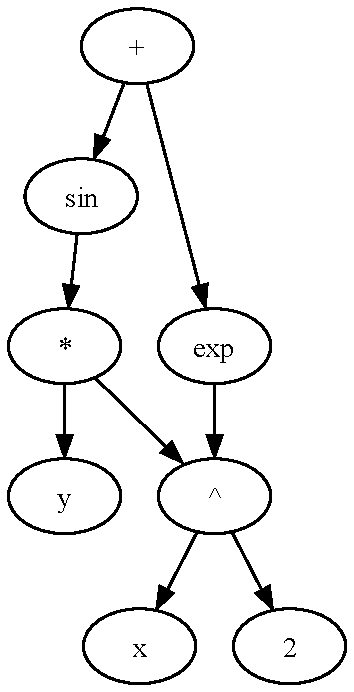
\includegraphics[width=4cm]{images/Graph_Example2.pdf}
    \caption{DAG of \eqref{example2}}
    \label{fig:DAGgraph}
\end{figure}

\subsection{Example of Forward Mode}

\begin{algorithm}[h]
\caption{ForwardmodeAD algorithm}\label{forwardAD}
\begin{algorithmic}[1]
\Procedure{ForwardmodeAD}{$expression,conditions$}
\State dict = dict()\Comment{}
\For{each $symbol$ in conditions}
    \For{each node i in expression}\Comment{By postorder traversal, operands before element}
    \State Calculate $v_i$ and $\Dot{v_i}$ w.r.t its $\varphi_i(v_j)_{j \prec i}$ \verb|operands| and \verb|symbol|
    \State dict[symbol] = \verb|expression.adjoint|\Comment{Store the adjoint w.r.t the symbol}
    \EndFor
\EndFor
\State \textbf{return} a dictionary of symbols and their respective \verb|adjoints|
\EndProcedure
\end{algorithmic}
\end{algorithm}

\subsection{Example of Reverse Mode}

Say we want to apply our algorithm to \eqref{example2} represented by the DAG in Figure \ref{fig:DAGgraph} evaluating at $x=2$, $y=2$. Here we label the nodes according to the notation used above as seen in Table \ref{example1}. 

We then traverse the graph in postorder traversal, computing the value of each node as we go along. The results after this pass are seen in Table \ref{tab:example1FP}. Now we will traverse the tree with preorder traversal. We know that first $\dot{v_6} \equiv 1$ and we have all our values calculated from the previous pass, so we get the adjoints as listed in Table \ref{tab:example1RP}


\begin{table}[h!]
    \centering
    \begin{tabular}{|lcl|lclll|}
        \hline
        $v_{-1}$ & $\equiv$ & $x$ & $\Bar{v}_{-1}$ & $=$ & $\Bar{v_2}\frac{\partial{v_2}}{\partial{v_{-1}}}$ & $=$ & $\Bar{v_2}v_1 {v_{-1}}^{(v_{1}-1)}$\\
        $v_{0}$ & $\equiv$ & $y$ & $\Bar{v}_{0}$ & $=$ & $\Bar{v_3}\frac{\partial{v_3}}{\partial{v_0}}$ & $=$ & $\Bar{v_3}v_2$\\
        \hline
        $v_{1}$ & $=$ & $2$ & $\Bar{v}_{1}$ & $=$ & $\Bar{v_2}\frac{\partial{v_2}}{\partial{v_1}}$ & $=$ & $\Bar{v}_{2}{v_{-1}}^{v_{1}}\log(v_{-1})$\\
        $v_{2}$ & $=$ & ${v_{-1}}^{v_{1}}$ & $\Bar{v}_{2}$ & $=$ & $\Bar{v_3}\frac{\partial{v_3}}{\partial{v_2}} + \Bar{v_5}\frac{\partial{v_5}}{\partial{v_2}}$ & $=$ & $\Bar{v}_{3}v_0 + \Bar{v_5}e^{v_2}$\\
        $v_{3}$ & $=$ & ${v_{0}}*{v_{2}}$ & $\Bar{v}_{3}$ & $=$ & $\Bar{v_4}\frac{\partial{v_4}}{\partial{v_3}}$ & $=$ & $\Bar{v_4}\cos(v_2)$\\
        $v_{4}$ & $=$ & $\sin(v_3)$ & $\Bar{v}_{4}$ & $=$ & $\Bar{v_6}\frac{\partial{v_6}}{\partial{v_4}}$ & $=$ & $\Bar{v_6}$\\
        $v_{5}$ & $=$ & $e^{v_2}$ & $\Bar{v}_{5}$ & $=$ & $\Bar{v_6}\frac{\partial{v_6}}{\partial{v_5}}$ & $=$ & $\Bar{v_6}$\\
        \hline
        $v_{6}$ & $=$ & $v_5 + v_4$ & $\Bar{v}_{6}$ & $=$ & $\frac{\partial{v_6}}{\partial{v_6}}$ & $=$ & $1$\\
        \hline
    \end{tabular}
    \caption{Table of Node Values and Adjoints in Figure \ref{fig:DAGgraph} of \eqref{example2}}
    \label{tab:example1}
\end{table}

\begin{table}[h!]
    \centering
    \begin{tabular}{|lclllcl|}
        \hline
        $v_{-1}$ & $=$ & $x$ & $\equiv$ & 2 & $=$ & 2\\
        $v_{0}$ & $\equiv$ & $y$ & $\equiv$ & 2 & $=$ & 2\\
        \hline
        $v_{1}$ & $\equiv$ & $2$ & $=$ & 2 & $=$ & 2\\
        $v_{2}$ & $\equiv$ & ${v_{-1}}^{v_{1}}$ & $=$ & $ 2^2$ & $=$ & $4$\\
        $v_{3}$ & $\equiv$ & $v_0 * v_2$ & $=$ & $ 2 \cdot 4$ & $=$ & $8$\\
        $v_{4}$ & $\equiv$ & $\sin(v_3)$ & $=$ & $\sin(8)$ & $\approx$ & $0.9894$\\
        $v_{5}$ & $\equiv$ & $e^{v_2}$ & $=$ & $ e^4$ & $\approx$ & $54.5982$\\
        \hline
        $v_{6}$ & $\equiv$ & $v_5 + v_4$ & $=$ & $e^4 + \sin(8)$ & $\approx$ & $55.5875$\\
        \hline
    \end{tabular}
    \caption{Values of Figure \ref{fig:DAGgraph} After Forward Pass}
    \label{tab:example1FP}
\end{table}


\begin{table}[h!]
    \centering
    \begin{tabular}{|lclll|}
        \hline
        $\Bar{v}_{6}$ & $=$ & $1$ & $=$ & $1$ \\
        \hline
        $\Bar{v}_{5}$ & $=$ & $\Bar{v_6}$ & $=$ & $1$\\
        $\Bar{v}_{4}$ & $=$ & $\Bar{v_6}$ & $=$ & $1$\\
        $\Bar{v}_{3}$ & $=$ & $\Bar{v_4}\cos(v_3)$ & $=$ & $1 \cdot \cos(8) = \cos(8)$ \\
        $\Bar{v}_{2}$ & $=$ & $\Bar{v}_{3}v_0 + \Bar{v_5}e^{v_2}$ & $=$ & $\cos(8) \cdot 2 + 1 \cdot e^{4} = 2\cos(8)+e^4$ \\
        $\Bar{v}_{1}$ & $=$ & $\Bar{v}_{2}{v_{-1}}^{v_{1}}\log(v_{-1})$ & $=$ & $4(2\cos(8)+e^4)\log(2)$ \\
        \hline
        $\Bar{v}_{0}$ & $=$ & $\Bar{v_3}v_2$ & $=$ & $\cos(8)\cdot4 = 4\cos(8)$ \\
        $\Bar{v}_{-1}$ & $=$ & $\Bar{v_2}v_1 {v_{-1}}^{(v_{1}-1)}$ & $=$ & $(2\cos(8)+e^4) \cdot 2 \cdot 2^{2-1} = 8\cos(8)+4e^4$ \\
        \hline   
    \end{tabular}
    \caption{Adjoints of Figure \ref{fig:DAGgraph} After Reverse Pass}
    \label{tab:example1RP}
\end{table}
From Table \ref{tab:example1RP} we get expressions for the partial derivatives given in \eqref{example1RPresults}.
\begin{equation} \label{example1RPresults}
    \begin{gathered}
    \frac{\partial F}{\partial y} = \Bar{v}_0 =  4\cos(8) \approx -0.58200013523 \\
    \frac{\partial F}{\partial x} = \Bar{v}_{-1} = 8\cos(8) + 4e^4 \approx 217.228599862
    \end{gathered}
\end{equation}

\newpage
\section{Implementation of Scalar Reverse Mode in Python}

To implement reverse mode AD in Python we used the symbolic language that we defined in \cite{PoPBook} as a template. This allowed us to have a symbolic language that we could use to easily construct our expressions. It does this by operator overloading our elementary operators so we can easily create an expression that we can traverse. Here we added additional elementary functions Sin, Cos, Exp and Log. So that they can exist in expressions we create and behave correctly. We also modified our base Expression class to contain the following attributes
\begin{verbatim}
    class Expression:
        def __init__(self, *operands):
            self.operands = operands
            self.storedvalue = 0
            self.adjoint = 0
\end{verbatim}
This allows us to store the intermediate value of our element as we traverse our DAG in our forward pass to use when calculating the adjoints in our reverse pass.
We also modified the \verb|evaluate()| function from \cite{PoPBook} to include evaluation of our functions Sin, Cos, Exp and Log. As an example here is the code for our evaluate method when our expression is Sin()
\begin{verbatim}
    @evaluate.register(expressions.Sin)
    def _(expr, *o, **kwargs):
        return np.sin(o[0])
\end{verbatim}

Then we have to create an algorithm for traversing and evaluating the DAG at each node. Note here we need to traverse the DAG in postorder traversal, where we visit the operands before we visit the element. Note in implementation we keep a dictionary of the expression and the stored value so we can avoid unnecessary calculation and to make the traversal non-recursive. The idea of the algorithm is seen in algorithm \ref{EvaluatePostvisitor}

\begin{algorithm}[h!]
\caption{EvaluatePostvisitor function}\label{EvaluatePostvisitor}
\begin{algorithmic}[1]
\Procedure{EvaluatePostvisitor}{$expression,conditions$}
\For{each element in expression}\Comment{Postorder traversal: visiting element after its operands}
\State \verb|value| $\gets$ \verb|evaluate(element, operands, conditions)|
\State \verb|element.storedvalue| $\gets$ \verb|value|
\EndFor
\EndProcedure
\end{algorithmic}
\end{algorithm}

Now that we have done a postorder traversal of our expression, each element contains a correct t\verb|element.storedvalue| attribute based on its elementary function and our evaluating conditions. Now we need to do a preorder traversal of our graph, evaluating the adjoint of each node. To do this we need to create a new \verb|adjoint_evaluate()| method similar to the previous \verb|evaluate()| method but instead it will calculate the adjoint of each of the operands with respect to the element, the Table \ref{tab:AdjEval} shows the output of \verb|adjoint_evaluate()| based on each element. Presume $w_1$ and $w_2$ are \verb|v_1.storedvalue| and \verb|v_2.storedvalue| respectively for $v_1$ and $c_2$ operands of \verb|element|. Note $\sin()$, $\cos()$, etc only have 1 operand and thus only 1 output

\begin{table}[h!]
    \centering
    \begin{tabular}{|lll|}
        \hline
        Type of \verb|element| & Operand 1  & Operand 2 \\
        \hline
        Add() & 1 & 1 \\
        Sub() & 1 & -1 \\
        Mul() & $w_2$ & $w_1$ \\
        Div() & $1/w_2$ & $-w_1/w_2^2$ \\
        Pow() & $w_2{w_1}^{(w_2-1)}$ & ${w_1}^{w_2}\log(w_1)$ \\
        Sin() & $\cos(w_1)$ &  \\
        Cos() & $-\sin(w_1)$ &  \\
        Exp() & $\exp(w_1)$ &  \\
        Log() & $1/w_1$ &  \\
        \hline
    \end{tabular}
    \caption{Output of \verb|adjoint\_evaluate(element)|}
    \label{tab:AdjEval}
\end{table}

Now we have our \verb|adjoint_evaluate()| method we can run this function at each element when traversing the expression tree in preorder traversal, visiting the element before its operands. The general idea of the algorithm is described in algorithm \ref{AdjointPrevisitor}

\begin{algorithm}[h]
\caption{AdjointPrevisitor function}\label{AdjointPrevisitor}
\begin{algorithmic}[1]
\Procedure{AdjointPrevisitor}{$expression$, adjoint=1}
\State \verb|expression.adjoint| $\gets$ adjoint
\State \verb|adjoint| $=$ \verb|adjoint_evaluate(expression, operands)|\Comment{adjoint is a list}
\For{each index,operand in enumerate(expressions.operand)}\Comment{Preorder traversal}
\State \verb|operand.adjoint| $+=$ \verb|adjoint[index]|$\cdot$ \verb|expression.adjoint|
\State run \verb|AdjointPrevisitor(operand, operand.adjoint)|
\EndFor
\EndProcedure
\end{algorithmic}
\end{algorithm}

Now we have populated all the elements with their respective adjoints and so we can simply return a dictionary of all the symbols and their adjoint values to get the derivatives of our original expression. So now we can simply define a new function to calculate the derivative of an expression given some conditions. The general idea of this function is seen in Algorithm \ref{reverseAD}

\begin{algorithm}[h]
\caption{ReversemodeAD algorithm}\label{reverseAD}
\begin{algorithmic}[1]
\Procedure{ReversemodeAD}{$expression,conditions$}
\State run \verb|EvaluatePostvisitor(expression, conditions)|
\State run \verb|AdjointPrevisitor(expression)|
\State \textbf{return} a dictionary of Symbols and their respective \verb|adjoints|
\EndProcedure
\end{algorithmic}
\end{algorithm}

Now we can test our implementation on the previous example given in \eqref{example2} represented by the DAG in Figure \ref{fig:DAGgraph}. To do this we run the code below. We see our output is exactly the same as we calculated previously.

\begin{verbatim}
    sin = expressions.Sin()
    exp = expressions.Exp()
    x = expressions.Symbol('x')
    y = expressions.Symbol('y')
    x2 = x**2
    expression = sin(y * x2) + exp(x2)
    conditions = {x:2, y:2}
    reversemodeAD(expression, conditions)
    > {'x': 217.22859986210804, 'y': -0.5820001352344542}
\end{verbatim}



\section{Accuracy of Results}

We can check the accuracy of our results using 2 methods, first, by using Taylor series we have the equation
\begin{equation}
    F(x + \epsilon) = F(x) + \frac{dF}{dx} \cdot \epsilon + \mathcal{O}(\epsilon ^ 2)
\end{equation}
When we send $\epsilon$ to 0 the term $\mathcal{O}(\epsilon)$ goes to 0 meaning we can find $\mathcal{O}(\epsilon^2)$ by rearranging the equation to get

\begin{equation}
    F(x + \epsilon) - F(x) - \frac{dF}{dx} \cdot \epsilon
\end{equation}

When we compute this we get a value for $\mathcal{O}(\epsilon^2)$ which as $\epsilon \longrightarrow 0$ $\mathcal{O}(\epsilon^2) \to 0$ at a rate proportional to $\epsilon^2$.

\begin{figure}[h!]
    \cite{finite}
    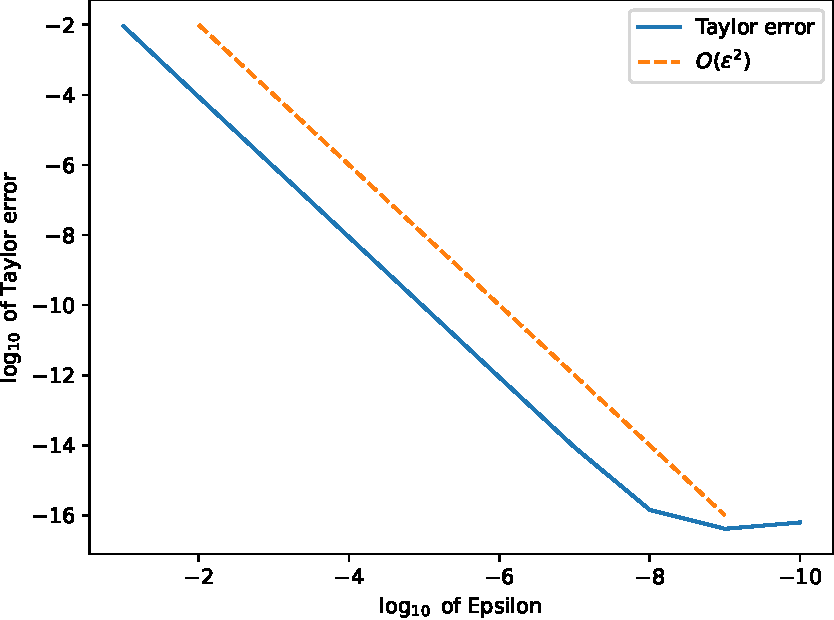
\includegraphics[width=12cm]{images/taylor_error_1.pdf}
    \caption{Plot of Taylor error against epsilon.}
    \label{fig:taylorerror}
\end{figure}

When checking if our result is correct we need to calculate the rate of convergence, since we are finding $O(\epsilon^2)$ we expect our convergence to be at the rate of $\epsilon^2$. To check our rate of convergence we use the formula:

\begin{equation}
    \frac{\log{\frac{\|u_1 - u\|}{\|u_2 - u\|}}}{\log{\frac{|h_1|}{|h_2|}}} = \frac{\log\|u_1 - u\| - \log\|u_2 - u\|}{\log|h_1| - \log|h_2|}
\end{equation}

Where $u_1, u_2$ are our approximations using $F(x + \epsilon) - F(x)$, $u$ is our calculated derivative using Reverse Mode AD, and $h_1, h_2$ are the corresponding $\epsilon$ for $u_1, u_2$. This value should give us the power of $\epsilon$ to which we are converging at. In our case we got:

\begin{center}
    \pgfplotstabletypeset[
    columns/0/.style={column name={Points}},
    columns/1/.style={column name={Gradients}},
    header=false,
    string type,
    before row=\hline,
    every last row/.style={after row=\hline},
    column type/.add={|}{},
    every last column/.style={column type/.add={}{|}}
]{images/rate_of_convergence.txt}%
\end{center}

As you can see at nearly all points we got values significantly close to 2. So we are converging at a rate of $\epsilon^2$.





\section{Extension and Implementation into NumPy Arrays}

Now we consider our expression as being a function of $F: \mathbb{R}^n \longrightarrow \mathbb{R}^m$. We cannot do this with our current implementation. Instead, we need to represent our expression as a NumPy 1 x m array, where each element of our array consists of the corresponding output. We can now change our algorithms for evaluation of the value and adjoint so they work correctly, this involves simply running our reversemode algorithm for each subexpression in our array, and making sure to record the adjoints of each of the symbols at each subexpresion. The modified algorithms are seen in Algorithm \ref{reverseADArr} and \ref{EvaluatePostvisitorArr}. Noting that our postvisitor traversal we use is still non-recursive.

\begin{algorithm}[h]
\caption{ReversemodeAD algorithm for arrays}\label{reverseADArr}
\begin{algorithmic}[1]
\Procedure{ReversemodeAD}{$expression,conditions$}
\State run \verb|EvaluatePostvisitor(expression, conditions)|
\For{each subexpression in expression}
\State run \verb|AdjointPrevisitor(subexpression)|
\EndFor
\State \textbf{return} a dictionary of Symbols and their respective \verb|adjoints| for each subexpression
\EndProcedure
\end{algorithmic}
\end{algorithm}

\begin{algorithm}[h!]
\caption{EvaluatePostvisitor algorithm for arrays}\label{EvaluatePostvisitorArr}
\begin{algorithmic}[1]
\Procedure{EvaluatePostvisitor}{$expression,conditions$}
\For{each subexpression in expression}
\For{each element in subexpression}\Comment{Postorder non-recursive traversal}
\State \verb|value| $\gets$ \verb|evaluate(element, operands, conditions)|
\State \verb|element.storedvalue| $\gets$ \verb|value|
\EndFor
\EndFor
\EndProcedure
\end{algorithmic}
\end{algorithm}

Now we can compute the adjoints of our DAG in Figure \ref{fig:DAGgraph2} for \eqref{example1} using our modified code. Here we get the following result for initial conditions $x=1$, $y=\pi$, $z=1$:

\begin{verbatim}
    sin = expressions.Sin()
    exp = expressions.Exp()
    log = expressions.Log()
    x = expressions.Symbol('x')
    y = expressions.Symbol('y')
    z = expressions.Symbol('z')
    x2 = x**2
    expx2 = exp(x2)
    expression = np.array([log(z) * expx2, expx2 + sin(x2 * y)])
    conditions = {x:1, y:np.pi, z:1}
    reversemodeAD(expression, conditions)
    > {'x': [0.0, -0.846621650261496], 'y': [0, -1.0], 'z': [2.718281828459045, 0]}
\end{verbatim}

Which is what we would expect.



\newpage
\section{Difference in Runtime}

Lets say we want to plot the time taken to compute various functions of $n$ unique input variables, as seen in \eqref{TimeFunc}. We can compare the difference in runtime between our Forward Mode AD and Reverse Mode AD. To give us a more robust plot we compute the average time taken over many iterations. The results of this test is seen in Figure \ref{fig:TimeDiff}.
\begin{equation} \label{TimeFunc}
    \begin{gathered}
        f_i: \mathbb{R}^n \longrightarrow \mathbb{R} \quad x \in \mathbb{R}^n \\
        f_1(x) = \prod_{i=1}^n x_i  \quad f_2(x) = \prod_{i=1}^n \sin(x_i) \\
        f_3(x) = \prod_{i=1}^n \exp(x_i)  \quad f_4(x) = \prod_{i=1}^n \log(x_i)
    \end{gathered}
\end{equation}

\begin{figure}[h]
    \centering
    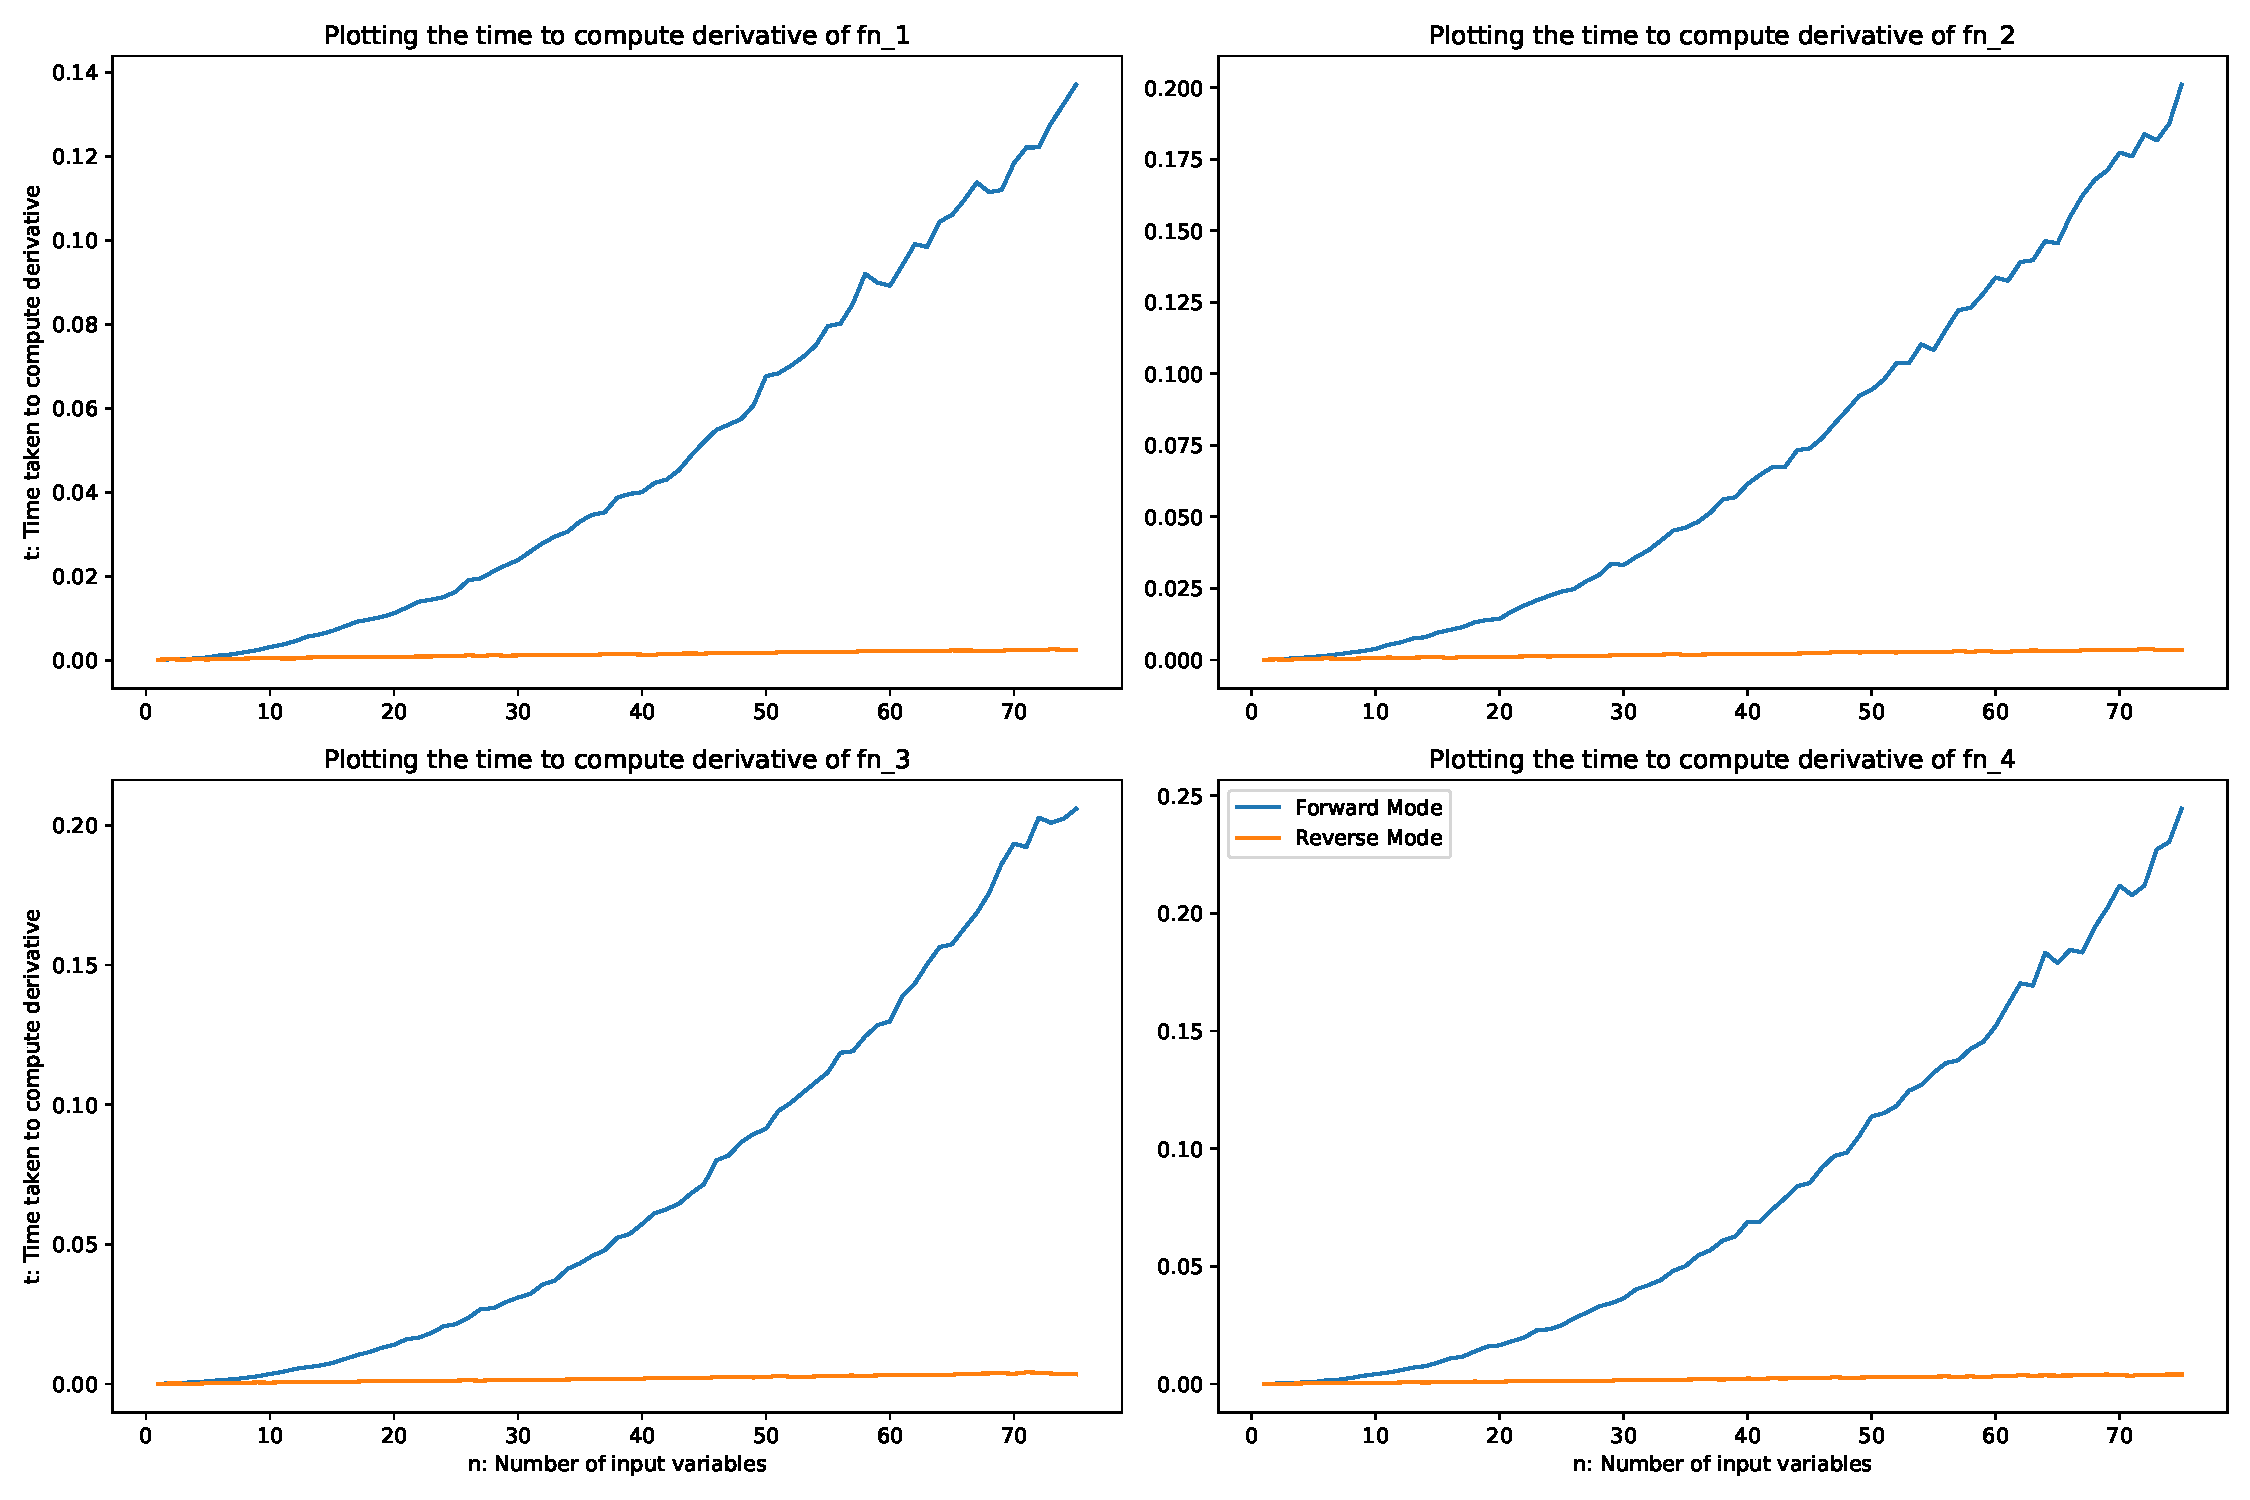
\includegraphics[width=15cm]{images/Graph_TimeDiff2.pdf}
    \caption{Average time taken to compute the derivatives of the functions in \eqref{TimeFunc} 50 times varying the number of input parameters}
    \label{fig:TimeDiff}
\end{figure}

As expected, Forward Mode automatic differentiation grows around linearly on the number of unique input variables that we have. This further proves the importance of using Reverse Mode automatic differentiation when working with systems with large amounts of variables like neural networks.

We can also see below the heatmap of the runtime when computing the derivative of a function, $F: \mathbb{R}^n \rightarrow \mathbb{R}^m$ listed in \eqref{func_nm}.

\begin{equation}
    F \begin{pmatrix}
        x_1 \\ \vdots \\ x_n
    \end{pmatrix} = \begin{pmatrix}
        \sum_{k=1}^n 1 \cdot x_k^1 \\ \sum_{k=1}^n 2 \cdot x_{k}^{2} \\ \vdots \\ \sum_{k=1}^n m \cdot x_{k}^{m}
    \end{pmatrix}
    \label{func_nm}
\end{equation}


\begin{figure}[h]
    \centering
    \includegraphics{images/Graph_HeatmapTimeDiff.pdf}
    \caption{Heatmap of mean time taken to compute the derivative of function in \eqref{func_nm}}
    \label{fig:heatmap}
\end{figure}

Here we can see that for a function with a low number of input parameters and high number of output variables we may prefer to use forward mode AD, however for functions with a high amount of input variables and a low number of output variables we will much prefer to use reverse mode AD. We can also see that reverse mode AD stays at low cost throughout compared to forward mode which blows up quickly with each increase in input/output variables



\newpage

\section{Implementing PDEs into Reverse Mode}

Currently we have implemented basic reverse mode algorithmic differentiation for general expressions. However what if we want to have a more complicated expression, perhaps one where one of our operators is to compute some PDE. This is our next extension we will be looking at. Paticularly we will be looking at solving and implementing the Advection-Diffusion equation into our current system.

\subsection{Advection Diffusion Equation}

Consider the simplified 1 dimensional advection-diffusion equation given by \eqref{AdvectionDiffusion} where we are measuring the concentration of some liquid over time, also accounting for the velocity of the liquid, $V$, and the rate of diffusion, $D$.

\begin{equation}
    \label{AdvectionDiffusion}
    \frac{\partial C}{\partial t} = - V\frac{\partial C}{\partial x} + D\frac{\partial^2 C}{\partial x^2}
\end{equation}

If we model concentration along the 1-dimension as a simple function of distance we can then interpolate the concentration across the domain. We have an example of interpolation of a function that denotes concentration distributed by the standard-normal distribution in Figure \ref{sampling:
\begin{figure}
\centering
    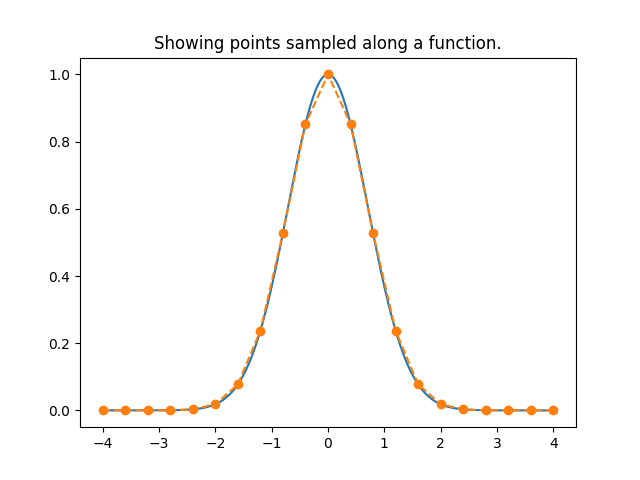
\includegraphics[width=12cm]{images/show_sampling.png}
    \caption{Difference between true function and sampled function}
    \label{fig:sampling}
\end{figure}

Now we have these points, using central difference equations, we can find approximations for $\frac{\partial C}{\partial x}$ and $\frac{\partial^2 C}{\partial x^2}$. If we number the nodes $C_1, \ldots , C_n$ then we get that:

\begin{equation}
    \frac{\partial C_i}{\partial x} \approx \frac{C_{i+1} - C_{i-1}}{2h}
\end{equation}
\begin{equation}
    \frac{\partial^2 C_i}{\partial x^2} \approx \frac{C_{i+1} -2C_i + C_{i-1}}{h^2}
\end{equation}

Where $h$ is the distance between each sample point. If we want to generalise this for all points we can use matrices like so:

\begin{equation} \label{CentralDifference}
    \begin{gathered}
        \underbrace{\frac{1}{2h}
        \begin{bmatrix}
        0 & 0 &  & & \\
        -1 & 0 & 1 & &\text{\huge{$0$}} & \\
         & -1 & 0 & \ddots &\\
         & & \ddots & \ddots & 1 \\
         & \text{\huge{$0$}} & & -1 & 0 & 1 \\
         & & & & 0 & 0
        \end{bmatrix}}_\text{\large{A}}
        \begin{bmatrix}
            C_1 \\ \vdots \\ C_n
        \end{bmatrix}
        \approx
        \begin{bmatrix}
            \frac{\partial C_1}{\partial x} \\ \vdots \\ \frac{\partial C_n}{\partial x}
        \end{bmatrix} \\
        \underbrace{\frac{1}{h^2}
        \begin{bmatrix}
        0 & 0 &  & & \\
        1 & -2 & 1 & &\text{\huge{$0$}} & \\
         & -1 & -2 & \ddots &\\
         & & \ddots & \ddots & 1 \\
         & \text{\huge{$0$}} & & -1 & -2 & 1 \\
         & & & & 0 & 0
        \end{bmatrix}}_\text{\large{B}}
        \begin{bmatrix}
            C_1 \\ \vdots \\ C_n
        \end{bmatrix} \approx
        \begin{bmatrix}
            \frac{\partial^2 C_1}{\partial x^2} \\ \vdots \\ \frac{\partial^2 C_n}{\partial x^2}
        \end{bmatrix}
    \end{gathered}
\end{equation}

Where the first and last row in the central difference matrix is all zeros as the derivative is 0 for the boundary conditions.
We denote the matrix for the first derivative as $A$ and the matrix for the second derivative as $B$. By stepping forward in time we get the equation.

\begin{equation}
    C_{\mathrm{new}} = C_{\mathrm{old}} + \Delta t \frac{\partial C_{\mathrm{new}}}{\partial t}
    \label{newC}
\end{equation}

We can approximate $\frac{\partial C}{\partial t}$ in \eqref{AdvectionDiffusion} by using $A, B$ denoted in \eqref{CentralDifference} and, then further plug this approximation into \eqref{newC} to get.
\begin{equation}
    \begin{split}
        & \frac{\partial C}{\partial t} \approx -VA + DB \\
        \Longrightarrow \ & C_{\mathrm{new}} = C_{\mathrm{old}} + \Delta t (-VA + DB) C_{\mathrm{new}} \\
        \Longrightarrow \ & [I + \Delta t(VA - DB)]C_{\mathrm{new}} = C_{\mathrm{old}}
    \end{split}
\end{equation}
Then defining $M$ as
\begin{equation}
    \begin{split}
        & M := I + \Delta t(VA - DB) \\
        \Longrightarrow \ &  C_{\mathrm{new}} = M^{-1} C_{\mathrm{old}}
    \end{split}
\end{equation}
Now solving this equation gives us a way of modelling the concentration in 1-dimension over time. Implementing this in Python and making use of the \verb|numpy.linalg| module we can easily do this.

\begin{figure}[h]
    \centering
    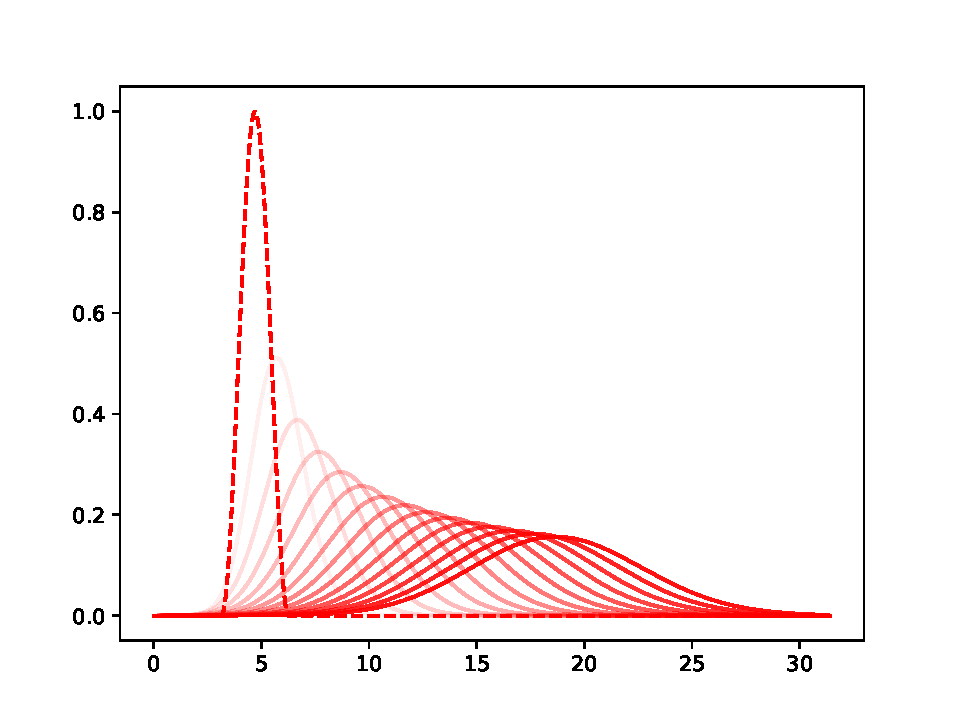
\includegraphics{images/Figure_1_ODE2.pdf}
    \caption{Plot of \eqref{AdvectionDiffusion} with V=10, D=5, plotting from t=0 to t=1.5 at timesteps of 0.1. Dotted line is value at t=0}
    \label{fig:ODE}
\end{figure}

\newpage

\bibliography{thebibliography}

\end{document}